\documentclass[18pt,caption=numbered]{beamer}
\usetheme[color=screen]{UniBern}

\usepackage{lmodern}
\usepackage[english]{babel}
\usepackage{microtype}
\usepackage{textcomp}
\usepackage[backend=biber, style=alphabetic, url=false]{biblatex}
\addbibresource{../../Documents/library.bib}
\usepackage{graphicx}
\usepackage{caption}
    \captionsetup[figure]{labelformat=empty} % No 'figure' in figures
\usepackage{tikz}
\usepackage[detect-all=true]{siunitx}
\usepackage{csquotes}
\usepackage{animate}
\usepackage{booktabs}
\usepackage[absolute,overlay]{textpos} %for the \source{} command
\usepackage{gitinfo2}
\usepackage{hyperref}

\hypersetup{pdfstartview={Fit}}
\setbeamertemplate{caption}{\insertcaption}
\setbeamertemplate{caption}[numbered]

\newcommand{\imsize}{\linewidth}
\newlength\imagewidth % needed for scalebars
\newlength\imagescale % ditto
\newcommand{\uct}{\si{micro}CT}

\newcommand{\source}[1]{%http://tex.stackexchange.com/a/48485/828
    \begin{textblock*}{4cm}(8.7cm,8.6cm)%
    \begin{beamercolorbox}[ht=0.5cm,right]{framesource}%
    \tiny\usebeamerfont{framesource}\usebeamercolor[fg]{framesource} Source: {#1}%
    \end{beamercolorbox}%
    \end{textblock*}%
}

% Biblatex: http://tex.stackexchange.com/a/13076/828
% % Format bibliography for beamer
% % http://tex.stackexchange.com/a/10686/828
% \renewbibmacro{in:}{}
% % http://tex.stackexchange.com/a/13076/828
% \AtEveryBibitem{\clearfield{title}}
% \AtEveryBibitem{\clearfield{journaltitle}}
% \AtEveryBibitem{\clearfield{year}}
% \AtEveryBibitem{\clearfield{pages}}
% \AtEveryBibitem{\clearfield{volume}}
% \AtEveryBibitem{\clearfield{number}}
% %http://tex.stackexchange.com/a/40710/828
% \usepackage{xpatch}
% \xpatchbibmacro{month}{%
%   \printtext[parens]%
% }{%
%   \setunit*{\addperiod\space}%
%   \printtext%
% }{}{} 

\subtitle{Brain and lung imaging as examples}
\author[DH]{David Haberthür}
\institute{Institute of Anatomy\\Universität Bern}
\date{February 9, 2017\\Internal seminar\\Version~\gitAbbrevHash}

\useoutertheme{split}

\begin{document}
\title[\si{\micro}CT imaging at ana.unibe.ch]{\si{\micro}CT-imaging at the Institute of Anatomy} % http://tex.stackexchange.com/a/144445/828

\defbeamertemplate{footline}{unibe}
{%
	\usebeamercolor[fg]{page number in head/foot}%
	\usebeamerfont{page number in head/foot}%
	\hspace*{\fill}%
	\insertauthor%
	\hspace*{\fill}%|\hspace*{\fill}%
	\insertshorttitle%
	\hspace*{\fill}%|\hspace*{\fill}%
	v.~\gitAbbrevHash%
	\hspace*{\fill}%|\hspace*{\fill}%
	\insertpagenumber\,/\,\insertpresentationendpage%
	\hspace*{\fill}%
	\vskip2pt%
}
\setbeamertemplate{footline}[unibe]

{
\setbeamertemplate{footline}{} % http://tex.stackexchange.com/a/18829/828
\begin{frame}
  \titlepage
\end{frame}
}
\addtocounter{framenumber}{1}

\begin{frame}{Contents}
	\tableofcontents
\end{frame}

\section{Overview}
\begin{frame}{Backstory}
    \begin{itemize}
        \item Lung fibrosis grading \cite{Ashcroft1988a}
        \item \emph{Correct} sampling for proper assessment
        \item \uct is a tool to help grade fibrosis
        \begin{itemize}
            \item Detect and grade fibrosis
            \item Get indications where to perform the sampling
        \end{itemize}
        \item Cancer metastasis (\SI{2}{year} after radiation treatment fibrosis is induced)
        \item Cancer treatment
        \begin{itemize}
            \item Antiangiogenesis (failed)
            \item Radiation therapy, namely MRT \cite{Bronnimann2016} (probably better citation needed)!
        \end{itemize}
    \end{itemize}
\end{frame}

\begin{frame}{Stories}
    \begin{itemize}
        \item  Overview of metastatis (Ochsenbein sample)
        \item Fibrosis grading (3View/uCT)
        \item Grenoble brains, assessing different parameters `easily'.
    \end{itemize}
\end{frame}

%\section{\uct}
\begin{frame}{Theory}
    \centering
    \begin{figure}
    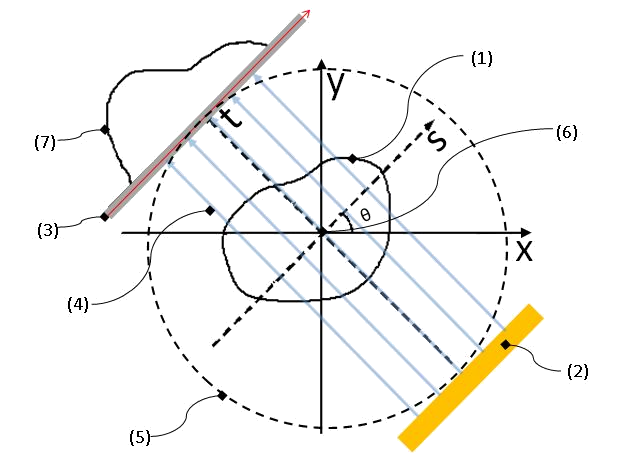
\includegraphics[width=0.5\linewidth]{img/CT_PRINCI_PB}
    \caption{Parallel beam CT.
        (1) = an object
        (2) = the parallel beam light source
        (3) = the screen
        (4) = transmission beam
        (5) = the datum circle
        (6) = the origin
        (7) = a one-dimensional fluoroscopic image}
    \end{figure}    
    \source{\href{https://commons.wikimedia.org/wiki/File:CT_PRINCI_PB.jpg}{enwp.org/tomography}}
\end{frame}

\section{Assessing metastasis load in lungs}
\begin{frame}{Lung metastasis}
    Show slide from anapath talk
\end{frame}

\begin{frame}{References}
    \renewcommand*{\bibfont}{\tiny}
    \printbibliography
\end{frame}

\end{document}

\begin{frame}{Machines}	
	\renewcommand{\imsize}{0.618\linewidth}
	\centering	
	\vfill
	\includegraphics[width=\imsize]{img/1272}
	\vfill
	\includegraphics[width=\imsize]{img/1172}
\end{frame}

\begin{frame}{Examples}
	\begin{itemize}
		\item Zebrafish
		\item Spider
		\item Lung tumors
	\end{itemize}
\end{frame}

\begin{frame}{Danio rerio}
\centering
\includegraphics[width=\imsize]{img/{{zebrafish_rec_voi_top_right}}}
%\begin{figure}%
%    \centering%
%    \pgfmathsetlength{\imagewidth}{\imsize}%
%    \pgfmathsetlength{\imagescale}{\imagewidth/1651}%
%    \def\x{1020}% scalebar-x starting at golden ratio of image width of 1651px = 1020
%    \def\y{391}% scalebar-y at 90% of image height of 434px = 391
%    \begin{tikzpicture}[x=\imagescale,y=-\imagescale]%
%        \node[anchor=north west, inner sep=0pt, outer sep=0pt] at (0,0) {\includegraphics[width=\imagewidth]{img/{{zebrafish_rec_voi_top_right}}}};
%        % 1615px = 35.48 > 100px = 2198um > 23px = 500um, 5px = 100um
%        %\draw[|-|,blue,thick] (20,154) -- (1634,127) node [sloped,midway,above,fill=white,semitransparent,text opacity=1] {\SI{35.487480000000005}{\milli\meter} (1615px) TEMPORARY!};
%        \draw[|-|,ultra thick] (\x,\y) -- (\x+234.19,\y) node [midway,above] {\SI{5}{\milli\meter}};
%    \end{tikzpicture}%
%    \caption{Visualization of a tomographic scan of a zebrafish, fixed in \SI{4}{\percent} PFA.}%
%\end{figure}%
\end{frame}

\begin{frame}
	\centering
	Examples
	 
\end{frame}

\end{document} 
